\documentclass[]{unswthesis}

%%% Class options:

%  undergrad (default)
%  hdr

%  11pt (default)
%  12pt

%  final (default)
%  draft

%  oneside (default for hdr)
%  twoside (default for undergrad)


%% Thesis details
\thesistitle{Vibration Diagnosis of Planetary Gearbox under Variable Speed Condition }
\thesisschool{School of Mechanical and Manufacturing Engineering}
\thesisschool{School of Mechanical and Manufacturing Engineering}
\thesisauthor{Hengcheng Zhang}
\thesisZid{z5130844}
%\thesistopic{XX00}  % for undergrad theses only
\thesisdegree{Master of Engineering in Mechanical Engineering}
%\thesisdegree{Doctor of Philosophy}
\thesisdate{October 2017}
\thesissupervisor{A/Prof.\ Zhongxiao Peng}% for undergrad theses only


%% My own LaTeX macros, definitions, etc
%%%% Shortcuts
\newcommand{\num}[2]{\mbox{#1\,#2}}			% num with units

%%%% Symbols
\newcommand{\yes}{\ensuremath{\surd}\xspace}		% Tick mark
\newcommand{\no}{\ensuremath{\times}\xspace}		% Cross mark
\newcommand{\by}{\ensuremath{\times}\xspace}		% XXX x XXX
\newcommand{\bAND}{\ensuremath{\wedge}\xspace}		% Bool. /\
\newcommand{\bOR}{\ensuremath{\vee}\xspace}		% Bool. \/
\newcommand{\becomes}{\ensuremath{\rightarrow}\xspace}	% -->

%%%% Custom environments

% Centered tabular with single spacing
\newenvironment{ctabular}[1]
    {\par\begin{sspacing}\begin{center}\begin{tabular}{#1}}%
    {\end{tabular}\end{center}\end{sspacing}}


%%%% Our default level for display in TOC - subsubsections
\setcounter{tocdepth}{2}



\begin{document}

%% pages in the ``frontmatter'' section have roman numeral page number
\frontmatter  
\maketitle

\chapter*{Abstract}\label{abstract}

Planetary gearboxes are widely used because of their large transmission ratio and high load resistance. Suddenly breakdown or failure could result in severe economic and safety losses. Thus an effective diagnosis method is of great importance. Despite the complexity of planetary gearboxes, extensive studies have been done on this area. But most of them are based on constant or narrow speed range applications. A wider speed range not only brings frequency change but also amplitude modulation caused by passage of resonance and torque change due to speed variation.

The experiment was carried out on UNSW planetary gearbox test rig. Three test sets are designed and one is performed on this stage. A promising diagnosis procedure is developed through literature review. It is firstly performing cepstrum modification to compensate resonance, then utilize order tracking to eliminate frequency modulation effects. At last TSA and Hilbert transform is performed to detect the fault frequency.

In test 1, the cepstrum exponential liftering method is proven effective to compensate resonance around 2 Hz of input shaft speed at 10 second. Since the vibration signal is dominated by the later high speed portion, signal from the last 10 seconds are processed and it effectively revealed the harmonics of planet gear fault frequency. As the impulse caused by gear fault is quite obvious in this test rig, Hilbert transform is more convenient and effective than TSA to detect the fault information. In the following stage, different fault types and larger speed fluctuation and wider speed range will be investigated. Then the effectiveness of this procedure will be validated.

\chapter*{Acknowledgements}\label{ack}

This work has been inspired by the labours of numerous academics in
the Faculty of Engineering at UNSW who have endeavoured, over the years, to
encourage students to present beautiful concepts using beautiful
typography.

Further inspiration has come from Donald Knuth who designed \TeX, for
typesetting technical (and non-technical) material with elegance and
clarity; and from Leslie Lamport who contributed \LaTeX, which makes
\TeX\ usable by mortal engineers.

John Zaitseff, an honours student in CSE at the time, created the
first version of the UNSW Thesis \LaTeX\ class and the author of the
current version is indebted to his work.

\chapter*{Abbreviations}\label{abbr}
\begin{description}
\item[BE] Bachelor of Engineering
\item[\LaTeX] A document preparation computer program
\item[PhD] Doctor of Philosophy
\end{description}


\tableofcontents
\listoffigures  % if required
\listoftables  % if required

%% pages in the ``mainmatter'' section have arabic page numbers and chapters are numbered
\mainmatter

\chapter{Introduction}\label{ch:intro}

The aim of this article is to investigate a method to identify planetary gearbox fault by vibration analysis. The planetary gearbox is 

Chapter~\ref{ch:literature} explains the background for this document.
Chapter~\ref{ch:style} states the style and submission related requirements
to theses submitted at the school.
Chapter~\ref{ch:content} explains content related requirements to theses.
Chapter~\ref{ch:eval} evaluates the thesis requirements template.  Finally,
Chapter~\ref{ch:conclusion} draws up conclusions and suggest ways to
further improve the thesis requirements template.


\chapter{Literature Review}\label{ch:literature}

In this chapter, some basic concepts and important knowledge are provided. These concepts are 

\section{Planetary Gearbox}

Planetary gearing or epicyclic gearing is a gear system typically consisting of four parts: sun gear, planet gear, ring gear and the planet carrier.

There are several input-output ways for planetary gearboxes, such as stationary ring gear, fixed carrier or no stationary part. The gear ratio of the planetary gearbox could be calculated as:

\begin{equation}
	N_s\omega_s + N_p\omega_p - (N_s + N_p)\omega_c = 0
\end{equation}
\begin{equation}
	N_r\omega_r - N_p\omega_p - (N_r - N_p)\omega_c = 0
\end{equation}

The following figure shows a typical planetary gearing system, which contains 3 planet gears.

\begin{figure}
	\centering
	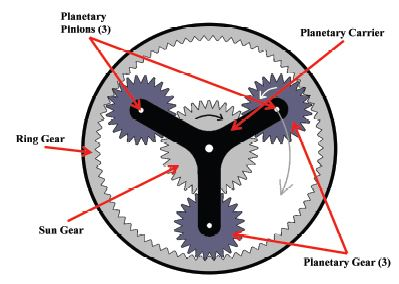
\includegraphics{PGB}
	\caption{Planetary gearbox layout \cite{gearbox}}
	\label{simulationfigure}
\end{figure}

The characters of planetary gearbox make it suitable for large transmission ratio, high load and split input or output circumstances. So it is widely used in wind turbines, lathes, vehicles and helicopters. The wide appliance and tough working environment of planetary gearbox require it to be highly dependable. Failures of planetary gearboxes may lead to huge economic losses as well as safety incidents. But the compact and complex structure, on the other hand, make it difficult to monitor its condition. Especially when the load and operating speed are varying. This project focuses on the varying speed conditions.


\section{Planetary Gearbox Fault Diagnosis}

The vibration of gear is caused by the geometric deviation of gears and teeth deformation under load. These two effects introduce a 'meshing error' or 'transmission error' (TE) \cite{vbcm}. The transmission error could be divided into three types: unloaded static TE, loaded static TE and dynamic TE. The unloaded static TE could be measured under a very light load, and it is realized to be caused by the geometric deviation. The load static TE is introduced by the tooth deflection under a constant load torque. Dynamic TE is caused by the fluctuation of torque and transmission speed.


\subsection{Vibration generated by gear}

Based on the understanding of transmission error, vibration generated by gears is classified as follows \cite{vbcm}:
\begin{enumerate}
\item Mean effects for all tooth pairs

The mean effects here are the same for all tooth pairs. Torque varies when each pair of teeth mesh and cause vibration. Therefore it is dominated by harmonics of tooth-mesh frequencies. It could be subdivided into three parts: 
\begin{itemize}
\item Tooth deflection due to mean torque.		
\item The mean part of initial profile errors resulting from manufacturing.		
\item Uniform wear over all teeth.
\end{itemize}
Uniform wear of teeth could increase friction force, which would result in higher harmonics of the gear mesh frequency.

\item Variation from the mean.

Variation from the mean could give rise to sidebands of harmonics and may be caused by:
\begin{itemize}
\item Slow variations, such as distortion and runout.		
\item Local faults, such as tooth spalls and root cracks.		
\item Random errors.		
\item Systematic errors.
\end{itemize}

Sidebands around the harmonics of gear mesh frequencies contain the gear fault information. The spaces between sidebands and harmonics show which gear has a fault, while the form of sidebands identifies the type of fault. For example, local faults may give rise to a flat sideband spectrum, while distributed fault may inspire higher level but narrowly grouped sidebands. 
Due to the limitation of time and resource, the fault investigated in this project is local faults, including tooth spalls and root cracks.
\end{enumerate}

Separation of spalls and cracks is another important topic due to the reason that cracks could cause a much more rapid failure. Endo \cite{Endo} developed a finite element analysis method to investigate their difference. It was found that cracks at tooth root give a two-stage deviation of transmission error due to the reason that at first stage, faulty tooth together with a healthy tooth share the load and at the second stage, faulty tooth stands the load alone. Spalls, on the other hand, inspire one deviation of TE when mating tooth passes the spall.  

\subsection{ Characteristic of planetary gearbox signals}

Comparing to fixed-axis gearbox, in which each gear rotates around a fixed center, planetary gearbox has planet gears which rotate around not only their own centers but also the center of the sun gear. The transmission structure of planetary gearbox brings unique behaviors \cite{review}.
\begin{enumerate}
	\item The planet gears are meshing simultaneously with the sun gear and the ring gear. Part of the vibrations excited by different component and their different meshing phases could be neutralized or canceled by each other.
	
	\item The multiple vibration transmission paths are time-varying and load effected in the planetary gearbox. It could attenuate the vibration signal of the defective part and weaken the fault characteristics.
	
	\item Differ from fixed-axis gearbox, sidebands appear in the spectrum for both healthy and faulty planetary gearboxes and asymmetric about the tooth-mesh frequency. It may be caused by multiple planet gears meshing with different phases.
	
	\item Vibrations of low-speed faulty components are easily masked and difficult to discover.
\end{enumerate}


\subsection{Diagnosis techniques}

As discussed in the former section, when gears are operating in good condition, the vibration signal tend to be stationary, containing gear mesh frequency and shafts rotating frequencies. When a fault happens, the amplitude or frequency components change according to the fault types.
Plenty of diagnosis techniques are developed to separate the faulty information from the original signal \cite{practical}.

\subsubsection{Statistic indicators}

Time domain statistical indicators are carried out directly from the vibration signal. Some of them are scaled including peak value, peak to peak value, mean value, root mean squared value and variance.
Among which RMS (root mean squared) value, as its name suggests, is the root of the mean of the squared signal values. It represents the overall vibration level. It is calculated as:
\begin{equation}
RMS = \sqrt{\frac{1}{N}\sum_{i=1}^n x_{i}^2}
\end{equation}

Variance indicates the power of the vibration, and its formula is:

\begin{equation}
\sigma^2 = \frac{1}{N}\sum_{i=1}^n (x_{i} - \overline{x})^2
\end{equation}

There are also some useful unscaled indicators, including kurtosis, crest factor and pulse factor. Kurtosis is the fourth moment normalized by the square of the mean square of the vibration signal waveform and represents the amplitude of impulse energy \cite{trending}.
\begin{equation}
K = \frac{\frac{1}{N}\sum_{i=1}^n (x_{i} - \overline{x})^4}{RMS^4}
\end{equation}

Crest factor shows impulse energy in another form:
\begin{equation}
C = \frac{x_{peak}}{RMS}
\end{equation}

Scaled indicators not only depend on the condition of the machine but also its running speed and load. Unscaled indicators have the benefit that they are independent of the running status.

\subsubsection{Time synchronous averaging}

TSA (Time synchronous averaging) is also a time domain signal processing method other than statistical indicators. It is implemented by averaging several segments of synchronizing signals together to extract the periodic signal from the background noises. It is calculated by:
\begin{equation}
y_{a}(t) = \frac{1}{N}\sum_{n=0}^{N-1} y(t+nT)
\end{equation}

The implementation of TSA depends on the corresponding of sample signals. Which means to be averaged numbers at each point should have the same rotating phase. This is guaranteed by 'Order tracking' method. When analyzing vibration signals of the rotating machines, a slight fluctuation of the rotating speed could cause smearing of the frequency components. Order tracking is making use of a shaft encoder signal or a tacho signal to resample the original signals with constant time interval into a constant phase interval signal. This method makes sure that the samples have same number and starting phase during each revolution. It is recommended to always perform order tracking before implementing TSA even at a constant speed.

The TSA method is firstly introduced into gear fault diagnosis by Stewart \cite{stewart}, whose propose to obtain the residual signal by removing the periodic gear meshing pattern and use the kurtosis of the residual signal as the fault indicator. Peter McFadden \cite{mc2} enhanced this method by improvements of the TSA as well as order tracking operations. He proposed to select a short section of signals which correspond to the vibration of one tooth and assembly together to the whole gear. Taking twice length of tooth mesh period signal sections with Hanning window was recommended to improve the frequency spectra in his later papers \cite{mc3}. Time synchronous averaged signals for a fixed period, normally one or two rotation of the shaft, would illustrate the fault type of the gear. As shown in Figure 2.2, plot a) is a steady gear mesh vibration. In plot b), the signal is amplitude modulated, which may be a consequence of misalignment. Plot c) is possibly because of significant wear of teeth surface, and plot d) may be caused by cracked tooth.

\begin{figure}
	\centering
	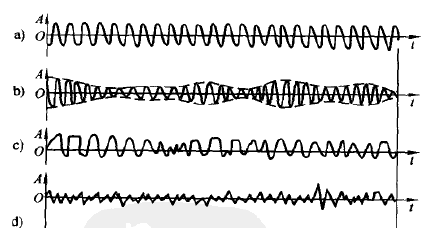
\includegraphics{TSA}
	\caption{Time synchronous averaged signals \cite{chen}}
	\label{tsa}
\end{figure}


\subsubsection{Frequency-domain methods}

Time-domain methods such as statistical indicators are able to find whether the gear is in malfunction, but not sufficient to the fault type.Frequency-domain methods are more capable of this requirement. They are developed based on Fourier transform. Under normal operating condition, the spectrum is dominated by shaft rotating and gear mesh frequency. Sidebands around them and their harmonics would identify the type of fault in some content as discussed in chapter 2.2.1.
More than Fourier transform or its implementation for the digital signal, DFT and FFT, demodulation techniques and cepstrum analysis are utilized to run the diagnosis.

As is already known that the faulty information of gears usually hides in the sidebands around gear mesh frequency and its harmonics, and these sidebands are mostly caused by amplitude and frequency modulation. Demodulation techniques such as Hilbert transform are effective to carry out the modulation signal. Thus it is able to investigate their faulty type and damage extent.
One example is introduced in \cite{mc4}. It uses Hilbert transform to demodulate the second harmonic of gear mesh frequency of the TSA signal. As seen in Figure \ref{demodulation}, the phase modulation signal of the TSA signal clearly shows the cracked tooth. It is even able to be known which tooth is in fault with certain phase information.

\begin{figure}
	\centering
	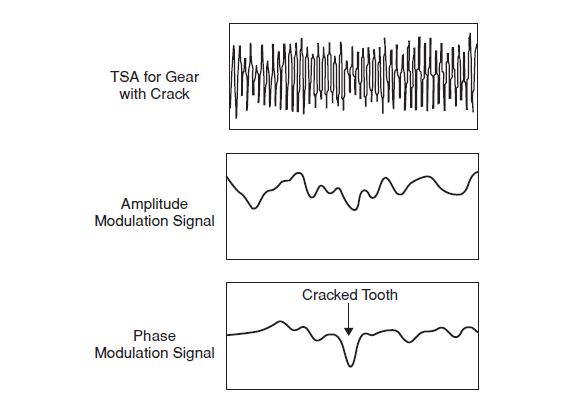
\includegraphics{demodulation}
	\caption{Demodulation of the second harmonic of the gearmesh frequency for a cracked gear \cite{mc4}}
	\label{demodulation}
\end{figure}

Cepstrum analysis is another important method to investigate the sidebands and transfer function. Cepstrum is the inverse Fourier transform of a logarithmic spectrum, which is Fourier transformed from a time signal. It is then:

\begin{equation}
\hat{x}(\tau) = IF[log(X(f))]
\end{equation}

Where $X(f)$ is the spectrum signal.

\subsubsection{Time-frequency-domain methods}

Time-frequency domain methods is a combination of time and frequency domains in one plot. Methods such as Wigner-Ville distribution and wavelets analysis are studied recently as another choice in vibration diagnostics. Meltzer \textit{et al.} \cite{mel1} \cite{mel2} conducted this method on an automobile planetary gearbox.


\section{Fault Diagnosis under Variable Speed Condtions}

Most of the methods mentioned in the former part are developed for constant speed and load conditions. When there are minor speed fluctuations, performing of order tracking would eliminate this effect. But when it comes to wider speed range, as much as $\pm$ 30 percent, besides frequency modulation, amplitude modulation caused by the passage of resonances, frequency response function and variation of torque comes into consideration. These effects could not be compensated by order tracking. Then the residual signal of TSA under these conditions would include much of the amplitude variation of the deterministic part as well as the random noise \cite{varyspeed}. One possible method is to find sections with relatively steady speed. Randall \cite{varyspeed} suggested another way to perform pre-processing of cepstrum modification to compensate the resonance part before order tracking and TSA.

\subsection{Cepstrum resonance compensation}

The cepstrum is obtained by inverse Fourier transform of the log spectrum. If the log spectrum includes phase part, it is complex cepstrum. If the log spectrum only has amplitude, then it is real or power cepstrum. The logarithmic conversion of the spectrum transforms the multiplication relationship between the forcing function and transfer function into an additive one \cite{vbcm}. It is also more evident to see the families of harmonics and sidebands in the log spectrum. Due to these characteristics, cepstrum analysis is able to be applied for collecting uniformly spaced sidebands and separating forcing functions from transfer functions.

In the variable speed gearbox diagnosis application, cepstrum is utilized to perform resonance compensation. Randall indicated in \cite{resonance} that low-quefrency region of the cepstrum is contributed by both excitation and transfer function, while the high -quefrency region is dominated by forcing function. So it is able to use liftering in cepstrum to remove the forcing function part, or on the contrary, remove the transfer function component. In \cite{varyspeed}, modal information is obtained by applying an exponential window to lifter the cepstrum. Removing the modal part in cepstrum and transfer back to spectrum and further to a time domain, it should be able to see a more uniform waveform. This means the amplitude variation due to passing resonances is compensated.

\subsection{Ordertracking and TSA}

Followed by the pre-processing of resonance compensation, 'order tracking' and TSA is now able to be performed. These two methods have already been discussed in chapter 2.2.3. Cepstrum modification removed the amplitude modulation caused by resonance. The next step is to deal with the phase modulation caused by varying speed. 'Order tracking' is a phase demodulation technique based on a reference phase-locked signal. It resamples the constant time interval signal to a constant phase increment signal. 'Order tracking' is used to avoid smearing of frequency components in its spectrum. Only after the application of order tracking, it is able to perform TSA.

As discussed in the former part, TSA is averaging together many signal segments corresponding to the same period of synchronizing signal. It is always performed for one or two rotation of the shaft. The averaged signal, as seen in Figures 2.2 and 2.3 would illustrate the fault in gears. A further investigation could be performed on the TSA or its residual signal. For example, the McFadden method /cite{McFadden} perform a more complicated TSA and check the Kurtosis of the residual signal. The Hilbert transforms technique \cite{mc4} could be performed to examine the amplitude and phase modulation signal as shown in Figure 2.3.

\section{Summary}

By reviewing of the literature above, it is acknowledged that vibration analysis of gearboxes has been widely researched. Planty of methods and techniques have been developed in this area. But most of these techniques are focused on fix axis gearboxes and constant speed conditions. Most of these methods fail to work for planetary gearboxes in varying speed conditions, which would be much more universal and widely performed. The complexity of planetary gearbox and amplitude modulation due to speed passing resonance bring a lot of challenge to this task. The suggested process is:

\begin{enumerate}
	\item Perform cepstrum modification for resonance compensation;
	
	\item Order tracking to avoid discrete frequency smearing due to the speed variation;
	
	\item TSA to investigate the fault.
	
\end{enumerate}

Vibration signal produced by gear fault is normally obvious. It could be shown as impulses at the waveform. It could be processed as a modulation signal in some extent. In this case, the third step of TSA is able to be replaced by Hilbert transform, which would reveal the fault frequency.












 \chapter{Methodology}\label{ch:methodology}

In this chapter, the test equipment and experiment procedures are presented. The experiment is based on the planetary test rig in UNSW. Vibration signals are collected by a National Instrument data acquisition system and analyzed in Matlab.

\section{Equipment}

The test equipment includes the planetary gearbox test rig, control system, and the data acquisition system.

\subsection{Planetary gearbox test rig}

The UNSW planetary gearbox test rig was firstly built by Sweeney in a parallel configuration and then modified to the planetary configuration. Seen from the layout in Figure 3.1, the test rig is driven by a 3 Phase AC induction motor and a hydraulic pump provided the resistance torque. Two flywheels are mounted on input and output shaft to minimize speed fluctuation.
Power is transferred through the planetary gearbox in the center. The planetary has a parallel stage and a planetary stage. The input of the parallel stage is a 42-tooth pinion gear, and the output is a 55-tooth spur gear fixed to the planet carrier. The planetary stage is driven by the planet carrier. It carries tree planet gears which have 23 teeth each. The ring is fixed and has 80 teeth. The output sun gear has 34 teeth.

\begin{figure}[h]
	\centering
	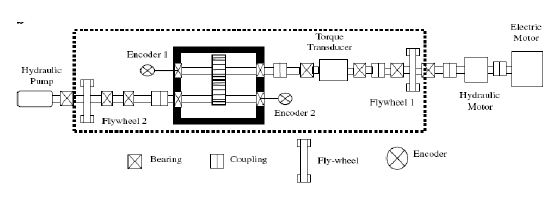
\includegraphics{rig}
	\caption{UNSW planetary gearbox test rig}
	\label{testrig}
\end{figure}

The gearbox is connected to the input and output shafts by belt couplings, which are not shown in the layout of Figure 3.1. The tension of the belts is adjusted by the sliding rails downside the gearbox housing. The planetary gearbox and the belt drives are illustrated in Figure 3.2.

An in-line torque transducer is used to measure the torque on the drive shaft. Its result is shown directly on The UNSW MK II transducer indicator. Due to the limitation of the belt transmission, the maximum torque is restricted to 70 Nm.
A Hidden 426-36000 shaft encoder is mounted on the input shaft of the gearbox. Which is shown in the upper-left corner of Figure 3.2. 
The external accelerometer is fixed by a stud to the outframe of the ring gear. There are two internal accelerometers, axial and radial, mounted inside the spur gear. The radial transducer rotates together with the carrier, and its signal is transferred out through a Michigan Scientific B6-2 slip ring on the left side. Both the external and internal transducers are Bruel \& Kjaer 4394 IEPE accelerometers.

\begin{figure}[h]
	\centering
	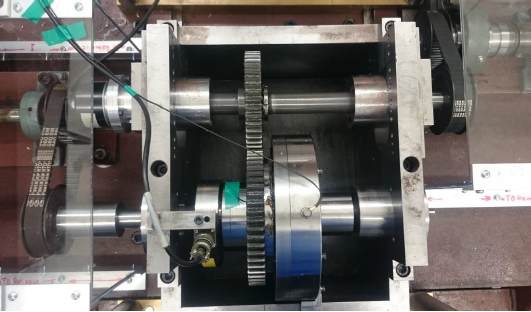
\includegraphics[scale = 0.7]{gearbox}
	\caption{The planetary gearbox}
	\label{gearbox}
\end{figure}

The speed of the AC induction motor is controlled by a FRENIC-MEGA variable frequency drive (VFD), which allows us to run the variable speed tests. As this is an 8 pole induction motor, the input frequency displayed on the variable frequency drive should be divided by four to get the drive shaft running frequency. The speed of the shaft could be controlled directly on the VFD using increase and decrease buttons or remotely controlled on the computer by the program. The VFD is what makes the variable speed test feasible.

The VFD is installed on the control panel together with its switch and an emergency stop button.  It also contains the hydraulic control valve and the hydraulic isolation valve. The resistance torque could be adjusted by the control valve. Two torque mode is provided: high torque and low torque. The control panel is shown in Figure 3.3.

\begin{figure}[h]
	\centering
	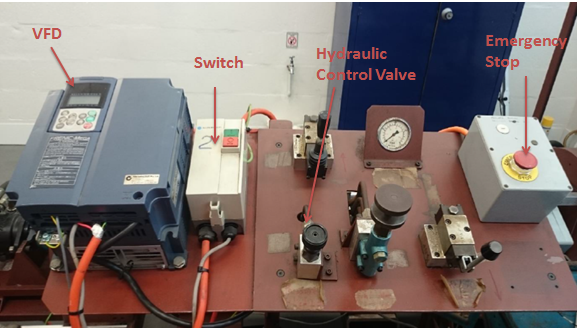
\includegraphics[scale = 0.7]{control}
	\caption{The control panel of the test rig}
	\label{control panel}
\end{figure}

\subsection{Data acquisition system}

The test signals generated by the rig are collected by a National Instrument (NI) PXI data acquisition system which is embedded with an internal PC. Data are collected and displayed through LabView. The collected data are finally processed in Matlab.

The PXIe-1071 system is an integrated data acquisition platform. It is widely used in machine monitoring, automotive and industrial test. The analog signal is conditioned and A/D converted by the data acquisition system and the digital signal is displayed and further processed in the computer. Chanel numbers of the PXI system is adjustable according to the chosen modules. It requires 2 vibration channel and one tacho channel to run this project.

\begin{figure}[h]
	\centering
	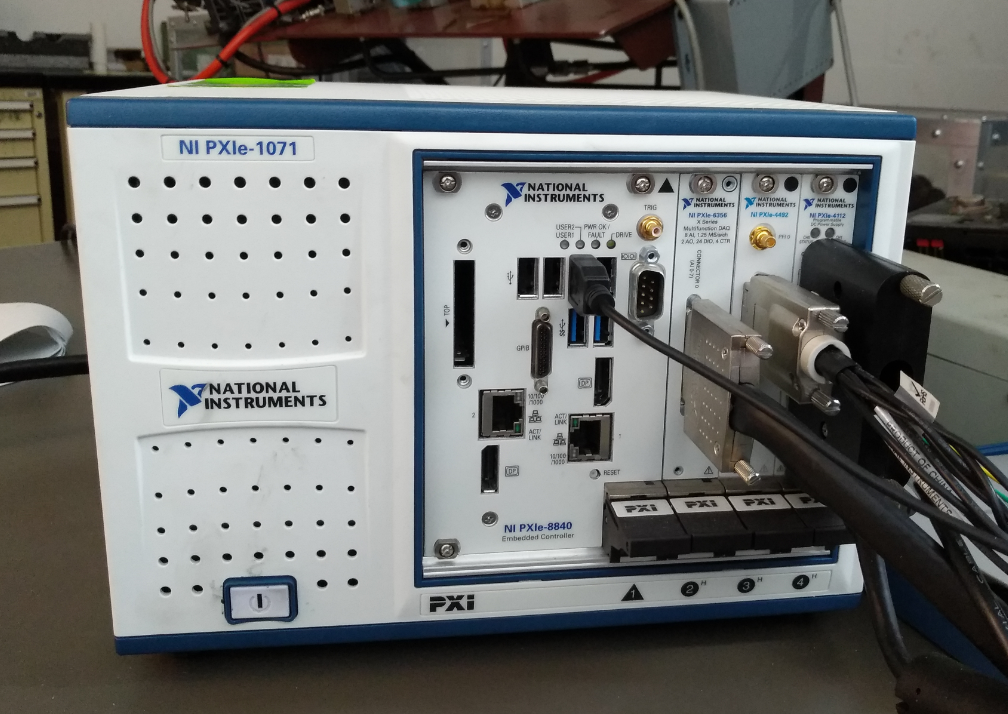
\includegraphics[scale = 0.4]{NI}
	\caption{The data acquisition system}
	\label{data acuisition}
\end{figure}

\section{Test Settings}

In this project, three test settings are conducted with the same gear fault. The first test is a speed up process in certain acceleration. The second test is a two-stage speed up process with different accelerations. The last is a speed fluctuation process. Comparisons are made to verify the developed diagnosis procedure.

\subsection{Test 1}

The first test is a run-up process. It starts at 1 Hz, which is 4 Hz on the variable frequency drive due to the 8-pole induction motor, and end at 6 Hz (24 Hz on VFD). The whole process takes 50 seconds and the shaft speed increase in a relatively constant acceleration. The load is set to be in low-loading mode. The speed profile is shown in the following figure. This test is to simulate the start-up process of the monitored machine. There could be a variety of incidents in the start-up stage, and a sooner detection of fault could prevent further damage effectively.

In this process, as the speed increases, the vibration amplitude increases accordingly. When it goes through resonance frequencies, even larger amplitude should be shown on its time domain waveform. This resonance could be compensated by performing of exponential liftering in theory.

\begin{figure}[h]
	\centering
	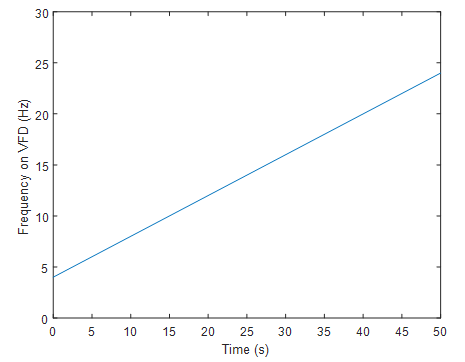
\includegraphics{speedup}
	\caption{Speed-up profile}
	\label{test1}
\end{figure}

\subsection{Test 2}

The speed profile of the second test is shown in Figure 3.6. It started from zero Hz and increased to 4 Hz (16 Hz on VFD) at a constant acceleration in 30 seconds. It stayed at this running speed for 20 seconds and went up to 6 Hz (24 Hz on VFD) in 30 seconds. The speed remained constant for another 20 seconds and then decreased to zero. This simulation is a whole process of the monitored machine from start-up to operation in different conditions and finally shut down.

During this test, seen from the speed profile, the accelerations are different in the two speed-up process and the slow-down process. The two constant speed platform would be analyzed as comparisons.

\begin{figure}[h]
	\centering
	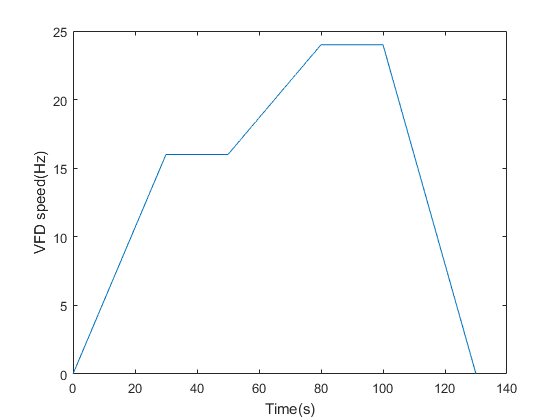
\includegraphics[scale = 0.85]{test2}
	\caption{Test 2 speed profile}
	\label{test2}
\end{figure}

\subsection{Test 3}

Many rotating machines such as automobile and wind generators operate in varying speed. Which brought challenges to the vibration based machine condition monitoring. In test 3, the varying speed process is simulated. The input shaft of the planetary gearbox was accelerated from zero to 5 Hz (20 Hz on VFD) in 30 seconds. Then it varies in a sinusoidal wave around 5 Hz for $\pm$25\%. After 4 cycles and 120 seconds, the machine was shut down to zero Hz. The speed profile of the whole process is shown below in Figure 3.7. This test is run on the low torque mode.

\begin{figure}[h]
	\centering
	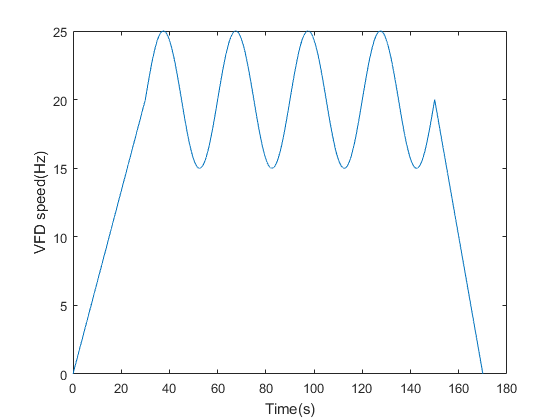
\includegraphics[scale = 0.85]{test3}
	\caption{Test 3 speed profile}
	\label{test3}
\end{figure}

\section{Processing and Analysis}

The data processing and analysis is extensively based on MATLAB. Data collected by NI PXI and LabView is stored in separate documents. It was first organized in MATLAB according to time and signal type. Each channel of the signal is stored as a vector. Additional messages such as torque and sample rate are supplied for further analysis. The investigated signal for our project is the external vibration and the tacho signal. The vibration signal holds the fault information of the gearbox, while the tacho gives running speed and phase information.

As discussed in chapter 2.4, the processing procedure is:

\begin{enumerate}
	\item Perform cepstrum modification for resonance compensation;
	
	\item Order tracking to avoid discrete frequency smearing due to the speed variation;
	
	\item Hilbert transform for demodulation.
	
\end{enumerate}

In this stage, only test 1 was performed, and all the processing and analysis is based on the data of test 1. The time domain vibration waveform from the external sensor is illustrated in Figure 3.8(1). As seen from the plot, the vibration amplitude increase according to the shaft speed. So the vibration signal is dominated by the largest last 10 seconds, which is shown in Figure 3.8(2).

\begin{figure}[htbp]
	\centering
	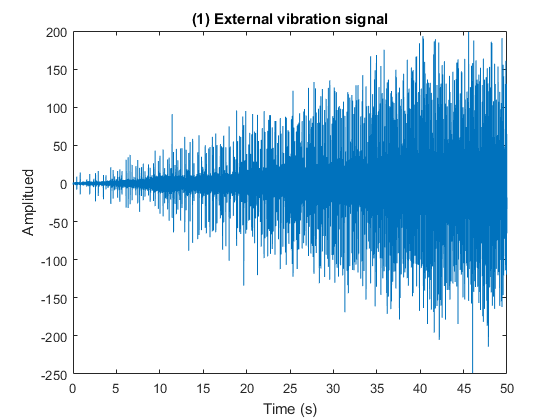
\includegraphics[scale =0.48]{wave}
	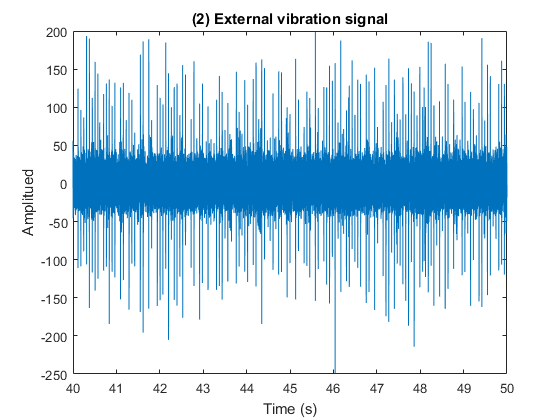
\includegraphics[scale =0.48]{last10}
	\caption{Vibration waveform of different period}
	\label{wave1}
\end{figure}

The first step, resonance compensation based on cepstrum modification, is performed on the signal of the whole period and that of the last 10 seconds. The liftered waveforms are shown as below:

\begin{figure}[h]
	\centering
	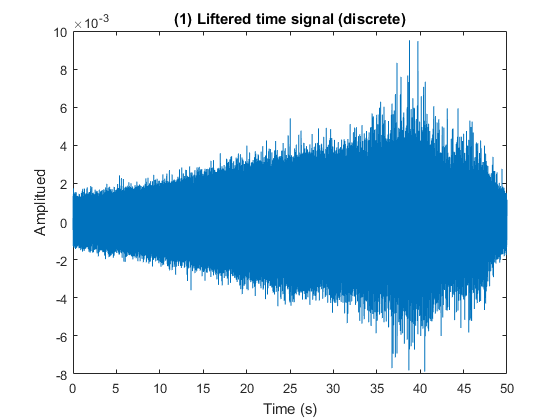
\includegraphics[scale =0.48]{wavelift}
	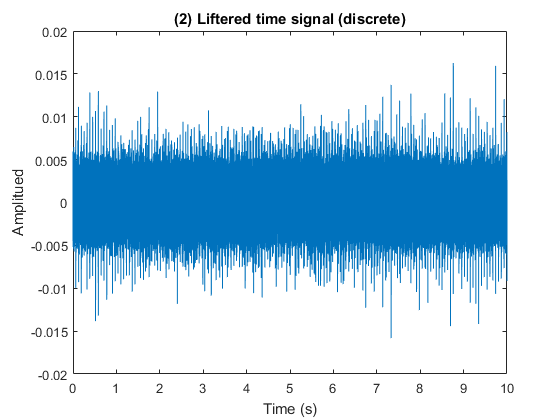
\includegraphics[scale =0.48]{last10lift}
	\caption{Liftered vibration waveform of different period}
	\label{wave2}
\end{figure}

Seen from Figure 3.8 and 3.9, the liftered signals are smaller and more uniform than the original ones. Looking into Figure 3.8 (1), it is able to be seen that there is an amplitude increase around 10 seconds. It could be the shaft passing through a resonance frequency. The liftered signal in Figure 3.9 (1), on the other hand, shows no other change besides the increasing along speed.

The second step is order tracking. This method is based on phase demodulation of the phase-locked tacho as a reference. A same number of samples are taken from each revolution. The order tracking method eliminates the effect of speed variation. When performing order tracking, the running speed is based on the tacho signal taken from the input shaft, and then transferred to carrier shaft speed by their gear ratio. Thus the carrier frequency is 1 Hz. Running frequency of other gears could be calculated based on it.

The last step is amplitude demodulation based on Hilbert transform. As discussed in the former part, the deterministic part of gear vibration is gear mesh signal. The shocks produced by gear fault are impulses in a lower frequency, which could be treated as amplitude modulation signal carried by the gear mesh frequency. In this condition, the Hilbert transform or envelope analysis is able to demodulate the faulty signal. At last, the spectrum of the amplitude information of the Hilbert transformed signal would reveal the faulty frequency. A comparison with each gear frequency would tell which one is with malfunction. 













\chapter{Evaluation}\label{ch:eval}

This chapter is mainly provided for the purpose of showing a typical thesis
structure.  There are no more thesis requirements described.

\section{Results}

The result of this work is the present document, being both a \LaTeX\
template and a thesis requirement specification.

\section{Discussion}

The Dual function of this document somewhat de-emphasises the primary
purpose of the document, namely the thesis requirements.  It would be
better, if these could be stated on a few concise pages (cf Appendix
1, p\pageref{app1}).

\chapter{Conclusion}\label{ch:conclusion}

\section{Conclusions}


\section{Future Work}





%% chapters in the ``backmatter'' section do not have chapter numbering
%% text in the ``backmatter'' is single spaced
\backmatter
\bibliographystyle{alpha}
\bibliography{pubs}
\begin{thebibliography}{99}
 \bibitem{pa} H.~Partl:\emph{German \TeX},TUGboat Volume~9, Issue~1 (1988)
 
 \bibitem{gearbox} National Research Council, \textit{Cost, Effectiveness, and Deployment of Fuel Economy Technologies for Light-Duty Vehicles},(2015)
 
 \bibitem{VBCM} Robert Bond Randall,\textit{Vibration-based Condition Monitoring - Industrial, Aerospace and Automotive Applications}, (2011) 
 
 \bibitem{review} Yaguo Lei, Jing Lin,\textit{ Condition monitoring and fault diagnosis of planetary gearboxes: A review}, Measurement, vol. 48, Feb. 2014
  
 \bibitem{McFadden} P.D.McFadden, I.M.Howard, \textit{The detection of seeded faults in an epicyclic gearbox by signal averaging the vibration}, Aeronautical Research Labs Melbourne, 1990
 
 \bibitem{Endo}  Endo, H. Randall, R.B. \textit{Differential diagnosis of spalls vs. cracks in the gear tooth fillet region} Journal of Failure Analysis and Prevention, 4(5), 57-65
 
 \bibitem{practical}  K. Ding, \textit{Practical Fault Diagnosis Techniques for Gears and Gearboxes }, 2005

 \bibitem{trending}  W. S. Siew, W. A. Smith, Z. Peng, and R. B. Randall,, \textit{Fault Severity Trending In Rolling Element Bearings}, presented at the Acoustics 2015 Hunter Valley, 2015.

 \end{thebibliography}

\chapter{Appendix 1}\label{app1}

This section contains the options for the UNSW thesis class; and
layout specifications used by this thesis.

\section{Options}

The standard thesis class options provided are:

\qquad
\begin{tabular}{rl}
undergrad & default \\
hdr & \\[2ex]
11pt & default\\
12pt &\\[2ex]
oneside & default for HDR theses\\
twoside & default for undergraduate theses\\[2ex]
draft & (prints DRAFT on title page and in footer and omits pictures)\\
final & default\\[2ex]
doublespacing & default\\
singlespacing & (only for use while drafting)
\end{tabular}

\section{Margins}

The standard margins for theses in Engineering are as follows:

\qquad
\begin{tabular}{|l|r|r|}
\hline
 & U'grad & HDR\\\hline
{\verb+\oddsidemargin+} & \unit[40]{mm} & \unit[40]{mm}\\
{\verb+\evensidemargin+} & \unit[25]{mm} & \unit[20]{mm}\\
{\verb+\topmargin+} & \unit[25]{mm} & \unit[30]{mm}\\
{\verb+\headheight+} & \unit[40]{mm} & \unit[40]{mm}\\
{\verb+\headsep+} & \unit[40]{mm} & \unit[40]{mm}\\
{\verb+\footskip+} & \unit[15]{mm} & \unit[15]{mm}\\
{\verb+\botmargin+} & \unit[20]{mm} & \unit[20]{mm}\\
\hline
\end{tabular}

\section{Page Headers}

\subsection{Undergraduate Theses}
For undergraduate theses, the page header for odd numbers pages in the
body of the document is:

\quad\fbox{\parbox{.95\textwidth}{Author's Name\hfill \emph{The title of the thesis}}}

and on even pages is:

\quad\fbox{\parbox{.95\textwidth}{\emph{The title of the thesis}\hfill Author's Name}}

These headers are printed on all mainmatter and backmatter pages,
including the first page of chapters or appendices.

\subsection{Higher Degree Research Theses}
For postgraduate theses, the page header for the body of the document is:

\quad\fbox{\parbox{.95\textwidth}{\emph{The title of the chapter or appendix}}}

This header is printed on all mainmatter and backmatter pages,
except for the first page of chapters or appendices.

\section{Page Footers}

For all theses, the page footer consists of a centred page number.  
In the frontmatter, the page number is in roman numerals.  
In the mainmatter and backmatter sections, the page number is in arabic numerals.
Page numbers restart from 1 at the start of the mainmatter section.  

If the \textbf{draft} document option has been selected, then a ``Draft'' message is also inserted into the footer, as in:

\quad\fbox{\parbox{.95\textwidth}{\hfill 14\hfill\hbox to 0pt{\hss\textbf{Draft:} \today}}}

or, on even numbered pages in two-sided mode:

\quad\fbox{\parbox{.95\textwidth}{\leavevmode\hbox to 0pt{\textbf{Draft:} \today\hss}\hfill 14\hfill\mbox{}}}

\section{Double Spacing}
Double spacing (actualy 1.5 spacing) is used for the mainmatter section, except for
footnotes and the text for figures and table.

Single spacing is used in the frontmatter and backmatter sections.

If it is necessary to switch between single-spacing and double-spacing, the commands \verb+\ssp+ and \verb+\dsp+ can be used; or there is a \verb+sspacing+ environment to invoke single spacing and a \verb+spacing+ environment to invoke double spacing if double spacing is used for the document (otherwise it leaves it in single spacing).  Note that switching to single spacing should only be done within the spirit of this thesis class, otherwise it may breach UNSW thesis format guidelines.

\section{Files}

This description and sample of the UNSW Thesis \LaTeX\ class consists of a number of files:

\quad\begin{tabular}{rl}
unswthesis.cls & the thesis class file itself\\[2ex]
crest.pdf & the UNSW coat of arms, used by \verb+pdflatex+ \\
crest.eps & the UNSW coat of arms, used by \verb+latex+ + \verb+dvips+ \\[2ex]
dissertation-sheet.tex & formal information required by HDR theses\\[2ex]
pubs.bib & reference details for use in the bibliography\\[2ex]
sample-thesis.tex & the main file for the thesis
\end{tabular}

The file sample-thesis.tex is the main file for the current document (in use,
its name should be changed to something more meaningful).  It presents
the structure of the thesis, then includes a number of separate files
for the various content sections.  While including separate files is
not essential (it could all be in one file), using multiple files is
useful for organising complex work.

This sample thesis is typical of many theses; however, new authors should
consult with their supervisors and exercise judgement.

The included files used by this sample thesis are:

\quad\begin{tabular}[t]{r}
definitions.tex \\
abstract.tex \\
acknowledgements.tex \\
abbreviations.tex \\
introduction.tex \\
background.tex
\end{tabular}
\quad\begin{tabular}[t]{r}
mywork.tex \\
evaluation.tex \\
conclusion.tex \\
appendix1.tex \\
appendix2.tex 
\end{tabular}

These are typical; however the concepts and names
(and obviously content) of the files making up the matter of the
thesis will differ between theses.

\chapter{Appendix 2}\label{app2}

This section contains scads of supplimentary data.

\section{Data}

Heaps and heaps and heaps and heaps and heaps and heaps of data.
Heaps and heaps and heaps and heaps and heaps and heaps of data.
Heaps and heaps and heaps and heaps and heaps and heaps of data.
Heaps and heaps and heaps and heaps and heaps and heaps of data.
Heaps and heaps and heaps and heaps and heaps and heaps of data.

Heaps and heaps and heaps and heaps and heaps and heaps of data.
Heaps and heaps and heaps and heaps and heaps and heaps of data.
Heaps and heaps and heaps and heaps and heaps and heaps of data.
Heaps and heaps and heaps and heaps and heaps and heaps of data.
Heaps and heaps and heaps and heaps and heaps and heaps of data.

Heaps and heaps and heaps and heaps and heaps and heaps of data.
Heaps and heaps and heaps and heaps and heaps and heaps of data.
Heaps and heaps and heaps and heaps and heaps and heaps of data.
Heaps and heaps and heaps and heaps and heaps and heaps of data.
Heaps and heaps and heaps and heaps and heaps and heaps of data.

Heaps and heaps and heaps and heaps and heaps and heaps of data.
Heaps and heaps and heaps and heaps and heaps and heaps of data.
Heaps and heaps and heaps and heaps and heaps and heaps of data.
Heaps and heaps and heaps and heaps and heaps and heaps of data.
Heaps and heaps and heaps and heaps and heaps and heaps of data.

Heaps and heaps and heaps and heaps and heaps and heaps of data.
Heaps and heaps and heaps and heaps and heaps and heaps of data.
Heaps and heaps and heaps and heaps and heaps and heaps of data.
Heaps and heaps and heaps and heaps and heaps and heaps of data.
Heaps and heaps and heaps and heaps and heaps and heaps of data.

Heaps and heaps and heaps and heaps and heaps and heaps of data.
Heaps and heaps and heaps and heaps and heaps and heaps of data.
Heaps and heaps and heaps and heaps and heaps and heaps of data.
Heaps and heaps and heaps and heaps and heaps and heaps of data.
Heaps and heaps and heaps and heaps and heaps and heaps of data.

Heaps and heaps and heaps and heaps and heaps and heaps of data.
Heaps and heaps and heaps and heaps and heaps and heaps of data.
Heaps and heaps and heaps and heaps and heaps and heaps of data.
Heaps and heaps and heaps and heaps and heaps and heaps of data.
Heaps and heaps and heaps and heaps and heaps and heaps of data.

Heaps and heaps and heaps and heaps and heaps and heaps of data.
Heaps and heaps and heaps and heaps and heaps and heaps of data.
Heaps and heaps and heaps and heaps and heaps and heaps of data.
Heaps and heaps and heaps and heaps and heaps and heaps of data.
Heaps and heaps and heaps and heaps and heaps and heaps of data.

Heaps and heaps and heaps and heaps and heaps and heaps of data.
Heaps and heaps and heaps and heaps and heaps and heaps of data.
Heaps and heaps and heaps and heaps and heaps and heaps of data.
Heaps and heaps and heaps and heaps and heaps and heaps of data.
Heaps and heaps and heaps and heaps and heaps and heaps of data.

Heaps and heaps and heaps and heaps and heaps and heaps of data.
Heaps and heaps and heaps and heaps and heaps and heaps of data.
Heaps and heaps and heaps and heaps and heaps and heaps of data.
Heaps and heaps and heaps and heaps and heaps and heaps of data.
Heaps and heaps and heaps and heaps and heaps and heaps of data.

Heaps and heaps and heaps and heaps and heaps and heaps of data.
Heaps and heaps and heaps and heaps and heaps and heaps of data.
Heaps and heaps and heaps and heaps and heaps and heaps of data.
Heaps and heaps and heaps and heaps and heaps and heaps of data.
Heaps and heaps and heaps and heaps and heaps and heaps of data.



\end{document}
